\section{RESULTADOS E DISCUSSÕES}

Nesta seção será discutido, da melhor maneira possível, os resultados obtidos causando as perturbações P1-P5 no sistema de refrigeração. Antes de iniciar o tópico da variação das temperaturas e pressões, é importante saber se as velocidades de rotação reais do compressor estão próximas do esperado durante o planejamento experimental. A tabela \ref{tab:Rotações Medidas} mostra as velocidades de rotação aferidas utilizando o tacômetro MDT-2238B. Nota-se que estas velocidades estão próximas das esperadas conforme as tabelas \ref{tab:pertubaçõesTransiente} e \ref{tab:pertubaçõesHisterese},logo, conclui-se que as condições de teste reais estão dentro do planejamento experimental esperado.

\begin{table}[htb]
    \centering
    \begin{tabular}{|c|c|}
        \hline
        \textbf{Perturbação} & \textbf{Frequência de Rotação Compressor Medida [RPM]} \\
        \hline
        P1 & 489 \\
        P2 & 838 \\
        P3 & 838 \\        
        P4 & 1083 \\
        P5 & 883 \\
        \hline
    \end{tabular}
    \caption{Velocidades de Rotação do Compressor Aferidas para as Perturbações P1-P5}
    \vspace{5pt} 
{\footnotesize Fonte: O Autor(2025) }
    \label{tab:Rotações Medidas}
\end{table}

\subsection{Perturbação pela Velocidade do Ventilador} \label{subsec:PertubaçãoVelVentilador}

A primeira observação, que talvez seja a mais específica entre todas, não observada de maneira tão clara, por exemplo, nas perturbações de rotação, são oscilações análogas às oscilações senoidais decrescentes até que o sistema estabilize em m determinado valor de temperatura ou pressão. Por exemplo, a figura \ref{fig:TempSucçãoSubidaeDescida} mostra o comportamento mencionado na temperatura de sucção e descarga do compressor nas perturbações P1 e P3.
\newpage
\begin{figure}[h]
    \centering
    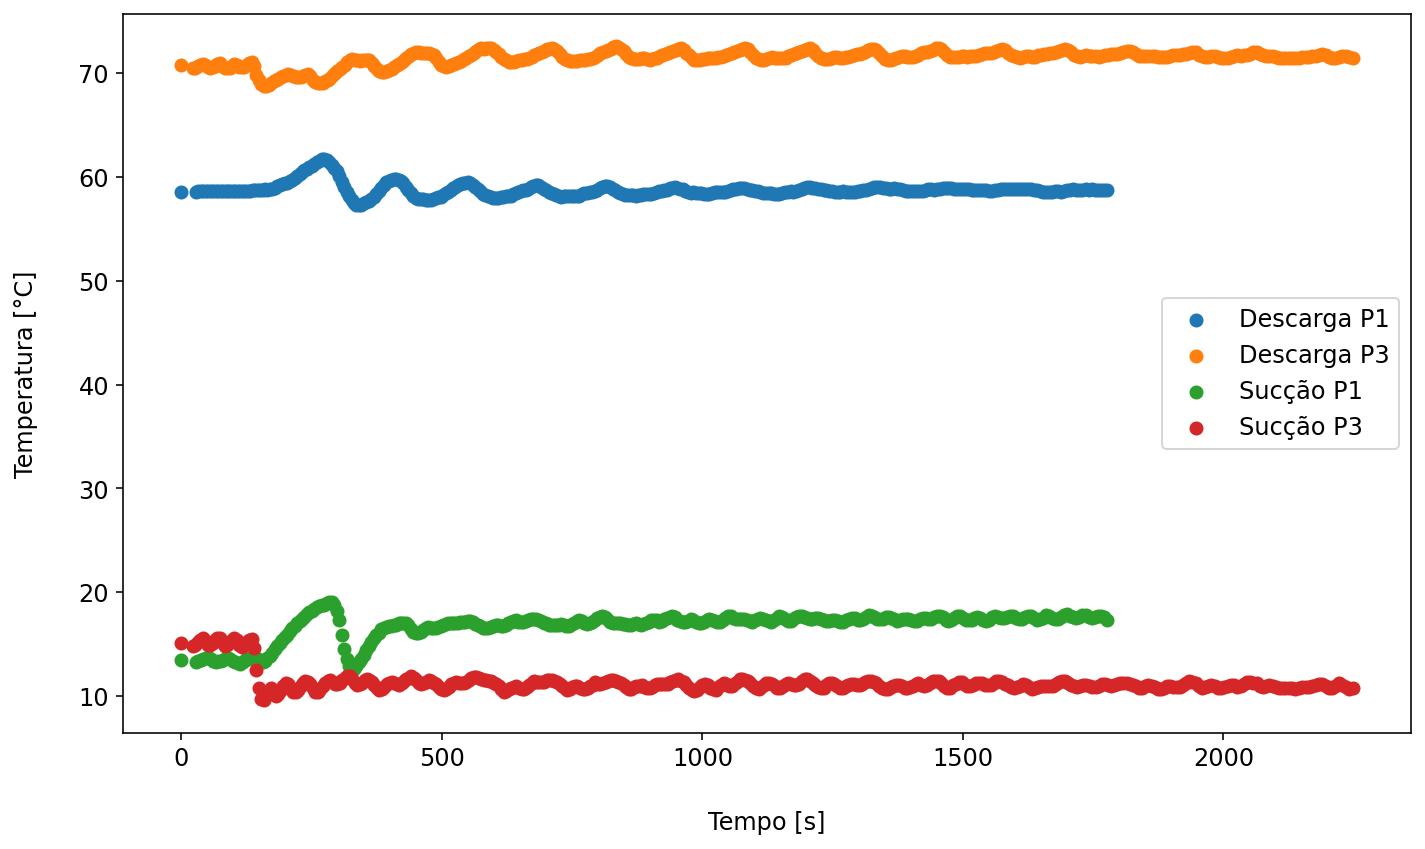
\includegraphics[width=1\linewidth]{FigurasdoTexto/Temperaturas de descarga e sucção Transiente P1 e P3.png}
    \caption{Temperaturas de Descarga e Sucção do Transiente de P1 e P3}
    \label{fig:TempSuccaoPertubacaoVentilador}
    {\footnotesize Fonte: O Autor (2025)}
\end{figure}

Nota-se, na figura \ref{fig:TempSuccaoPertubacaoVentilador}, que há um pico máximo de temperatura de sucção e descarga em P1 logo após o aumento da vazão de ar. Isto ocorre devido a um evaporador subalimentado \cite{StoekerRefrigeration}. Isto ocorre quando a válvula de expansão não consegue alimentar o evaporador com refrigerante o suficiente para refrigerar a superfície do evaporador adequadamente; como resultado, a temperatura e pressão sobem.

O pico mínimo de temperatura ocorre logo depois, provavelmente, ocorre devido a um evaporador inundado,isto é, após a subalimentação do evaporador, a válvula de expansão então deixa que mais fluido refrigerante passe até que o evaporador inunde, esta interpretação pode ser embasada com dados experimentais como na figura \ref{fig:VazãodeFluidoPerturbaçãoVentilador}, onde há um pico máximo de vazão de fluido refrigerante ao mesmo tempo em que as temperaturas de sucção e descarga são mínimas. Também, no artigo de \textcite{VaryingFanSpeedCavallaro} foi observado que aumentar a velocidade do ventilador implica em um aumento do coeficiente de transferência de calor h do sistema. Isto também deve estar auxiliando para que a queda da temperatura ocorra mais rapidamente.
\newpage
\begin{figure}[h]
    \centering
    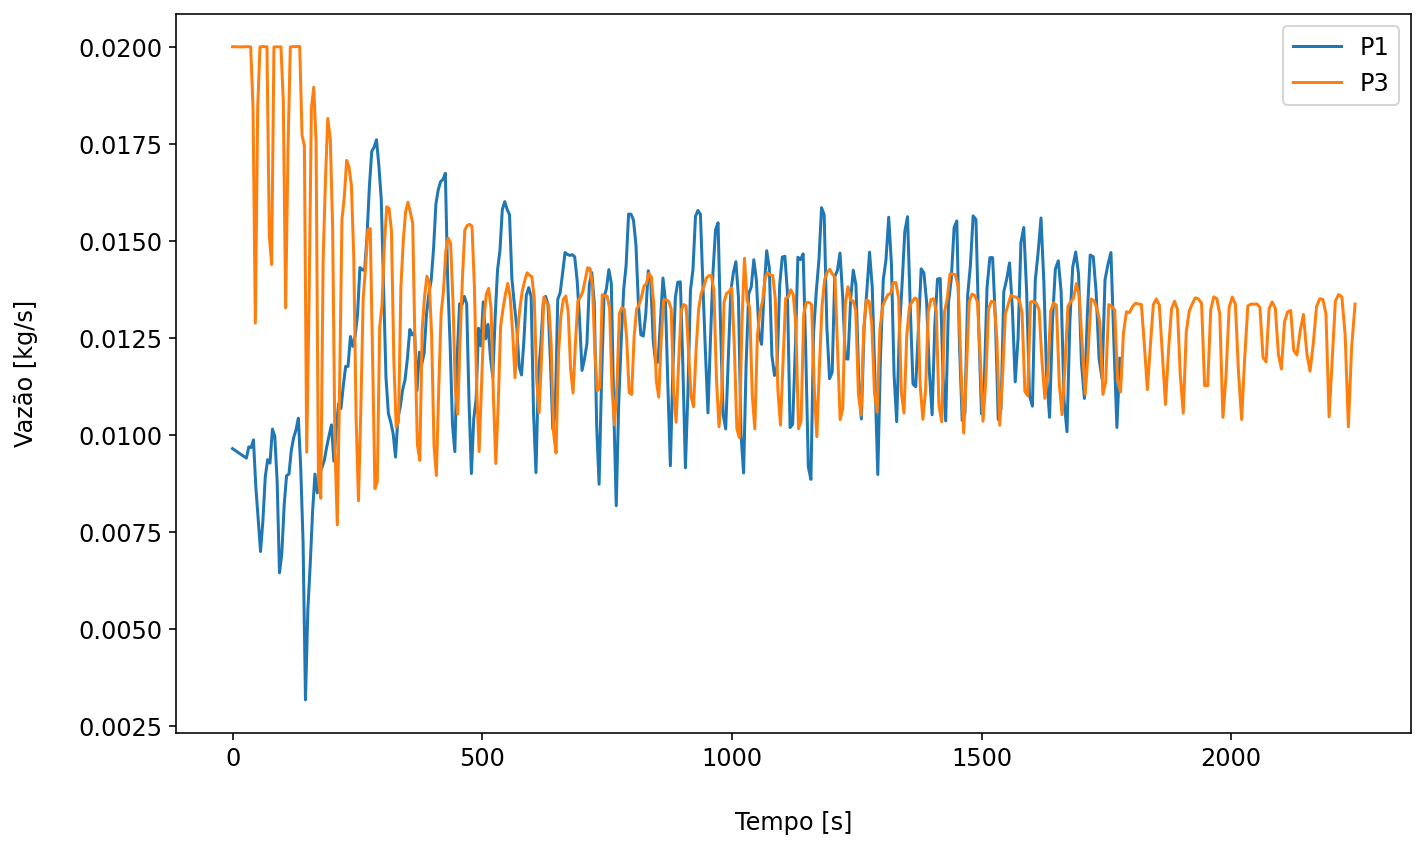
\includegraphics[width=1\linewidth]{FigurasdoTexto/VazãodeFluidoPerturbaçãoVentilador.png}
    \caption{Vazão de Fluído Refrigerante Transiente de P1 e P3}
    \label{fig:VazãodeFluidoPerturbaçãoVentilador}
    {\footnotesize O Autor (2025)}
\end{figure}
%Explicações- as temperaturas atingem um pico máximo devido a um evaporador seco (stoeker) causando aumento de temperatura e pressão e um pico mínimo de fluido vazão de fluido refrigerante. Já o mínimo ocorre devido a um evaporador cheio (inundado), faz sentido porque há um pico de vazão de fluido refrigerante .

No entanto, a temperatura após isso sobe, e oscila até estabilizar. Esta subida de temperatura possivelmente tem relação com que, embora o coeficiente de transferência de calor tenha aumentado,há mais massa de ar saindo do que o que pode ser resfriado de maneira mais eficaz pelo sistema, então as temperaturas sobem, e fazem isso oscilando, procurando a posição de equilíbrio entre a pressão de sucção e o fluxo da taxa de massa \cite{StoekerRefrigeration}.  

No caso de P3 não são observados extremos de temperatura, provavelmente pois, como a velocidade e vazão de ar neste caso são reduzidos, diminuí-los é uma alteração menos brusca no sistema, ela apenas decresce oscilando, devido possivelmente à mesma razão que P1 cresce, isto é, com menos vazão de ar é mais fácil resfriá-lo e oscila procurando o equilíbrio.

As pressões de descarga e sucção ambas crescem ou decrescem conjuntamente, o que é o oposto do observado nas pressões nas perturbações por rotação. Como na figura \ref{fig:Pressões de Sucção e Descarga P1 e P3},o aumento das pressões ou diminuição delas ocorre em decorrência do aumento ou diminuição da carga térmica no evaporador, respectivamente \cite{EffectsOFRefrigeranteCompressorAirFlow}.

\begin{figure}[h]
    \centering
    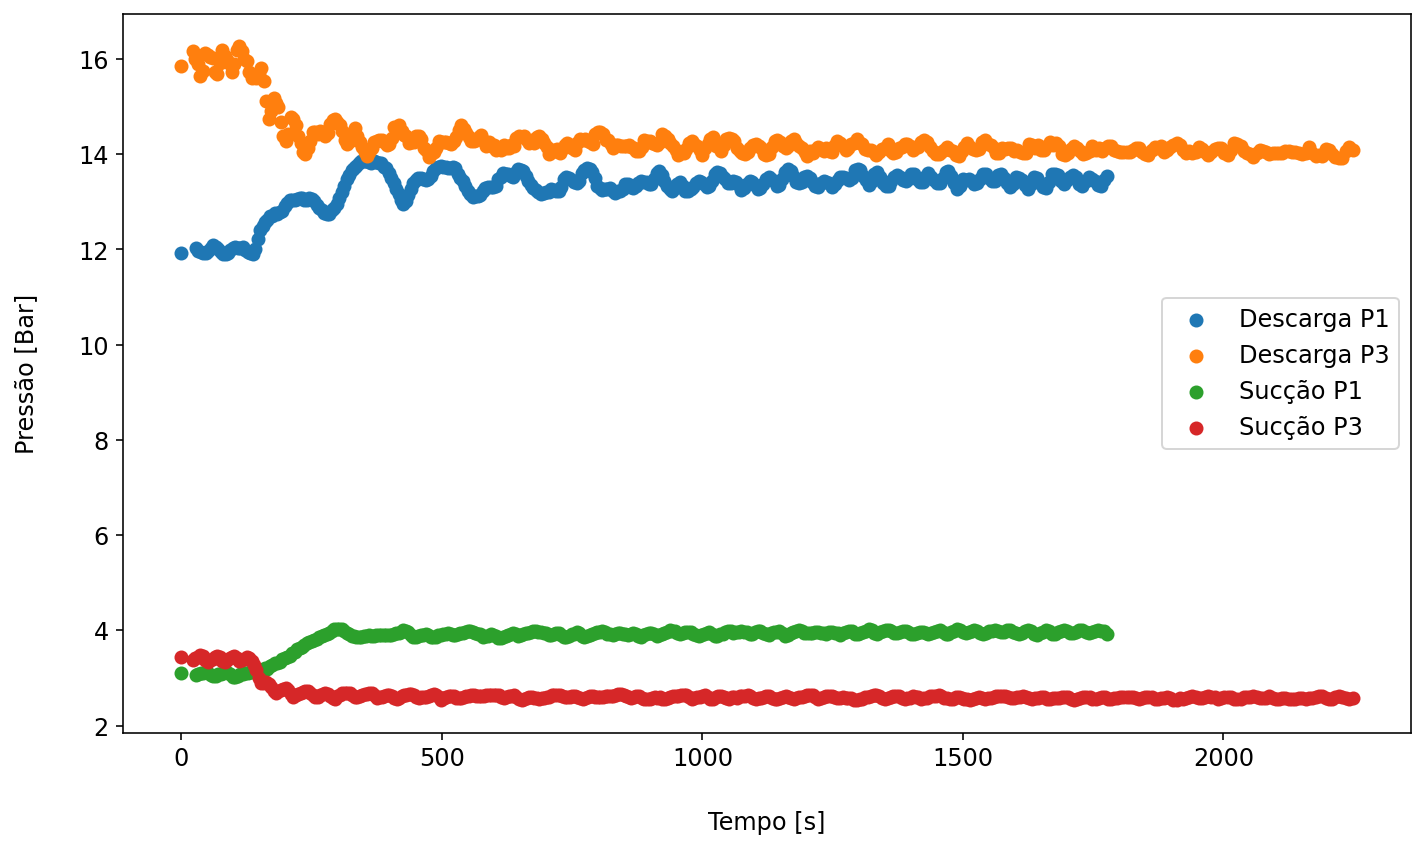
\includegraphics[width=1\linewidth]{FigurasdoTexto/Pressões de Sucção e Descarga P1 e P3.png}
    \caption{Pressões de Sucção e Descarga P1 e P3}
    \label{fig:Pressões de Sucção e Descarga P1 e P3}
    {\footnotesize O Autor (2025)}
\end{figure}

\subsection{Perturbação pela Frequência de Rotação do Compressor}


As perturbações causadas por rotação, como P2, P4 e P5, demonstraram um comportamento, em geral, menos oscilatório do que as que foram apresentadas previamente na subseção \ref{subsec:PertubaçãoVelVentilador}. É perceptível que, em relação às pressões, quando há aumento da velocidade de rotação do compressor, a pressão de descarga sobe e a de sucção desce, esta relação inversa entre as pressões também foi apontada em outros trabalhos, como o estudo de \textcite{EffectsOFRefrigeranteCompressorAirFlow}. Por exemplo, a figura \ref{fig:Pressão de Descarga e Sucção P2} mostra esta relação nas pressões de P2. 
\newpage
\begin{figure}
    \centering
    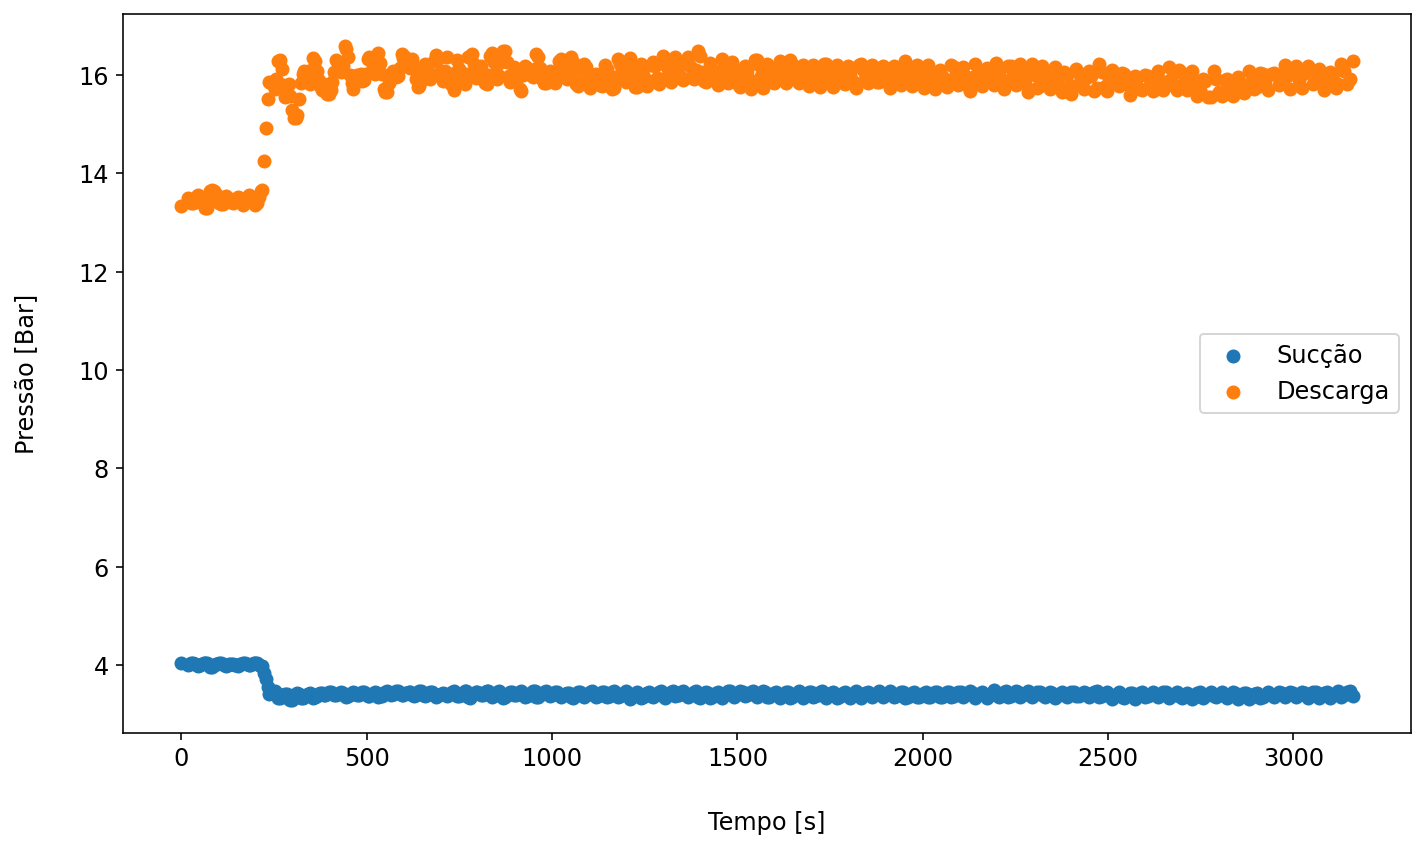
\includegraphics[width=1\linewidth]{FigurasdoTexto/Pressão de Descarga e Sucção P2.png}
    \caption{Pressão de Descarga e Sucção P2}
    \label{fig:Pressão de Descarga e Sucção P2}
    {\footnotesize O Autor (2025)}
\end{figure}

A relação inversa entre as pressões pode ser explicada devido à capacidade do compressor aumentar quando a rotação é elevada, variando então inversamente as quedas de pressão do diagrama P-V do compressor com o RPM ao quadrado \cite{phillippi2008basic}.
É observado também uma maior variação na pressão de descarga do que na pressão de sucção; tal comportamento ocorre devido ao aumento da região ocupada por líquido sub-resfriado no condensador. A prática é usual e serve à função de fazer com que apenas líquido entre na válvula de expansão \cite{StoekerRefrigeration},

O transiente da parte de sucção é mais rápido que na parte de descarga e isto é possível de concluir não somente das pressões, mas também das temperaturas respectivas, assim como mostra a figura \ref{fig:Temperaturas de Sucção e Descarga P2}. Esta diferente velocidade dos transientes ocorre, provavelmente, devido ao efeito da válvula de expansão. Ao aumentar a velocidade do compressor, a carga térmica aumenta quase que instantaneamente no sistema, isto aumenta a pressão e temperatura de descarga e mais  fluido refrigerante é sugado pelo compressor por consequência. No entanto, a válvula de expansão ainda demora para permitir que mais fluido refrigerante passe para o evaporador \cite{CHEN20081368}. Então, causando atraso, como visto na figura \ref{fig:Pressão de Descarga e Sucção P2} e \ref{fig:Temperaturas de Sucção e Descarga P2}. 

\begin{figure}[h]
    \centering
    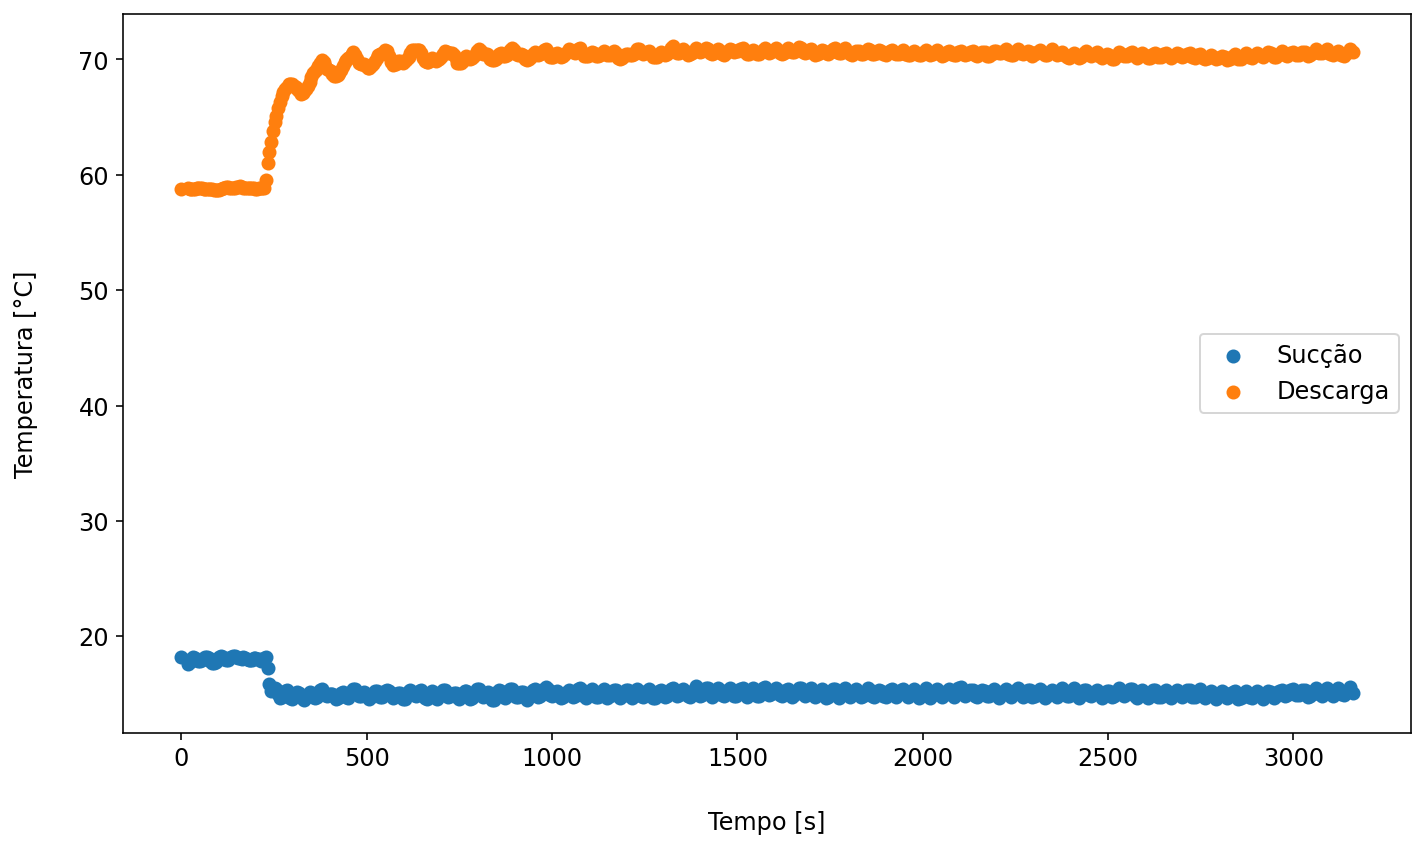
\includegraphics[width=1\linewidth]{FigurasdoTexto/Temperaturas de Sucção e Descarga P2.png}
    \caption{Temperaturas de Sucção e Descarga P2}
    \label{fig:Temperaturas de Sucção e Descarga P2}
    {\footnotesize O Autor (2025)}
\end{figure}
%\subsection{Estimativa dos Tempos de Acomodação}\newpage

\subsection{Análise da Histerese}

 Utilizando o método de análise introduzido na subseção \ref{subsec:Método de Análise da Histerese} deste trabalho,foi possível  calcular a histerese normalizada das principais variáveis do sistema de refrigeração. A figura \ref{fig:histereses normalizadas} demonstra então estes valores encontrados.
 \newpage
\begin{figure}[h] 
%gráfico a rever devido a valores maiores de histerese não antes analisados, mas creio que deve ter a ver com o que o lôndero falou da demora/rápidez conforme a mudança da válvula de expansão

%valores agora estão mais realistas, o problema é que estava comparando a entra e saída do 1002 com o 1001 e 1002 com 1004 o que não fazia sentido
    \centering
    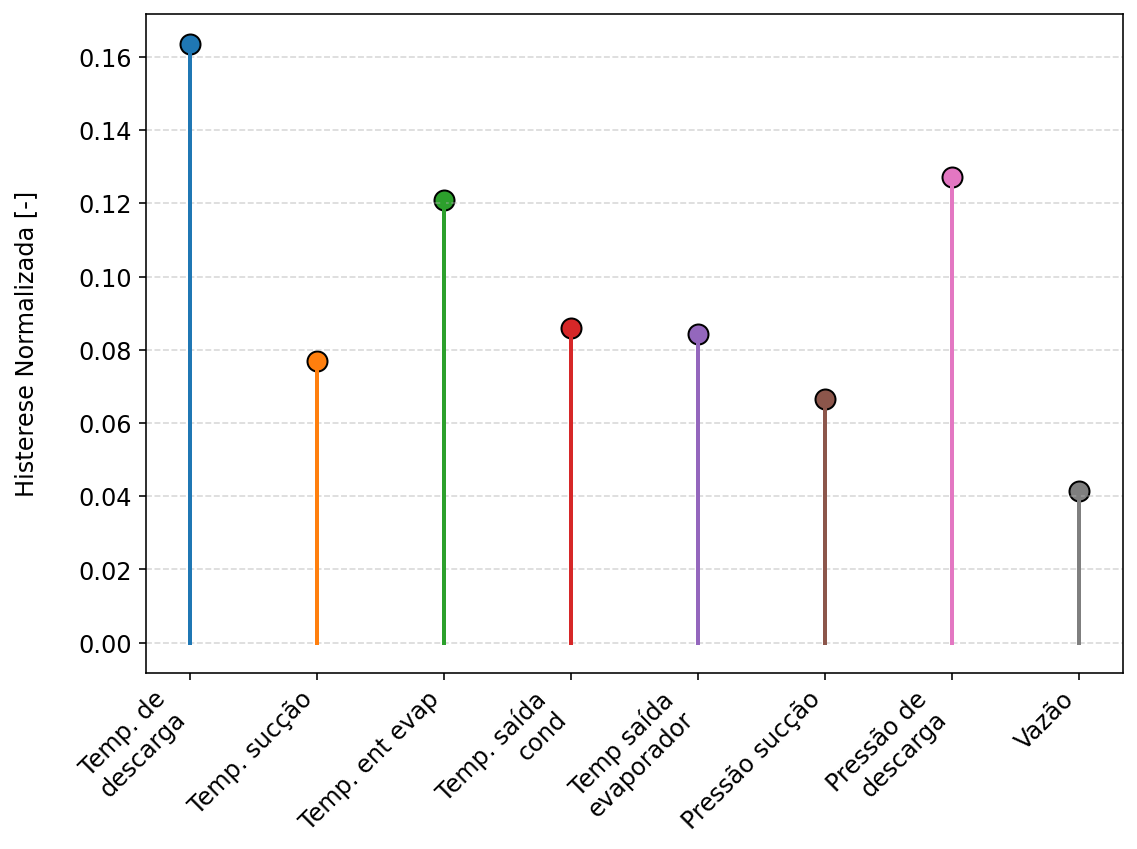
\includegraphics[width=1\linewidth]{FigurasdoTexto/Histereses Normalizadas.png}
    \caption{Histeres Normalizadas das Principais Variáveis do Teste}
    \label{fig:histereses normalizadas}
    {\footnotesize Fonte: O Autor(2025)}
\end{figure}

Nota-se que as histereses mais altas encontram-se próximas da região da válvula de expansão. Tanto na sua entrada como na sua saída, o que é um possível indício de que ela é a principal responsável pela diferença entre os caminhos de subida e descida de rotação. Foi também perceptível que a velocidade de convergência das variáveis de teste é afetada pela subida ou descida de rotação, principalmente das de menor histerese, como a temperatura e pressão de sucção. Por exemplo, o gráfico da figura \ref{fig:PressãodeSucçãoSubidaeDescida} mostra a pressão de sucção nas perturbações P4 e P5, nota-se que em boa parte do transiente na subida de rotação há uma lacuna na coleta dos dados. Isto acontece pois a subida do transiente foi mais rápida do que a taxa de amostragem do sistema de aquisição.
\newpage
\begin{figure}[h]
    \centering
    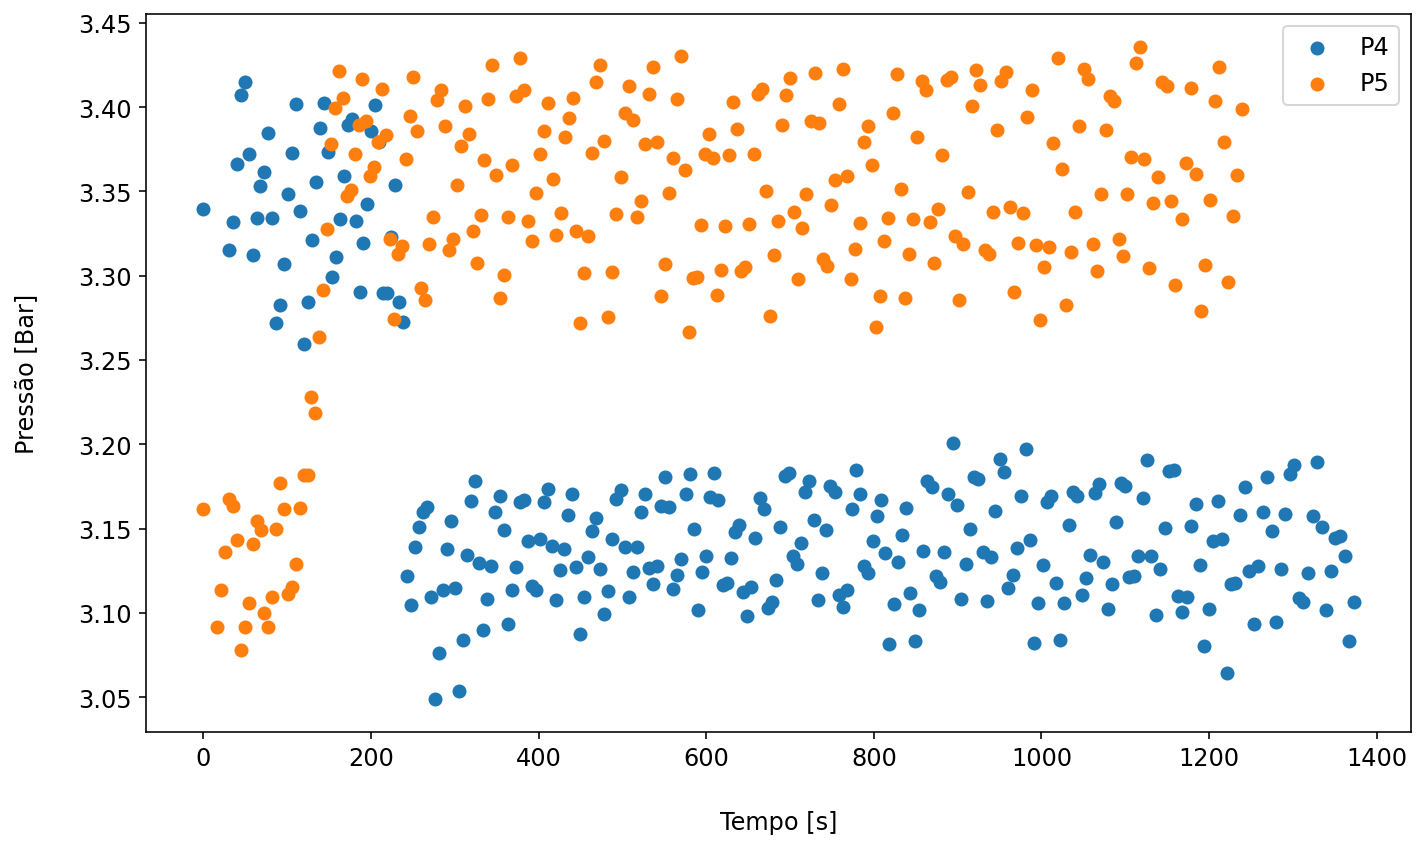
\includegraphics[width=1\linewidth]{FigurasdoTexto/Pressão de sucção subida e descida.png}
    \caption{Pressão de Sucção nas Perturbações P4 e P5}
    \label{fig:PressãodeSucçãoSubidaeDescida}
    {\footnotesize Fonte: O Autor(2025)}
\end{figure}

Uma possível explicação para esta mudança da velocidade de convergência pode ser o efeito da válvula de expansão. Quando a velocidade de rotação do compressor é diminuída, a vazão de fluido refrigerante passando pela válvula diminui, então ela começa a se fechar, não completamente, mas há diminuição da seção por onde passa o fluido, causando atraso no aumento da pressão de sucção. Contrastando com a situação oposta, isto é, durante o aumento da velocidade de rotação, há um aumento na vazão de fluido refrigerante, e a válvula já está completamente aberta, permitindo que a pressão varie mais facilmente. Tal comportamento é observável não só na pressão de sucção, mas também na temperatura, como mostra a figura \ref{fig:TempSucçãoSubidaeDescida}, o que demonstra que o comportamento citado acima é compatível com a observação experimental.

\begin{figure}[h]
    \centering
    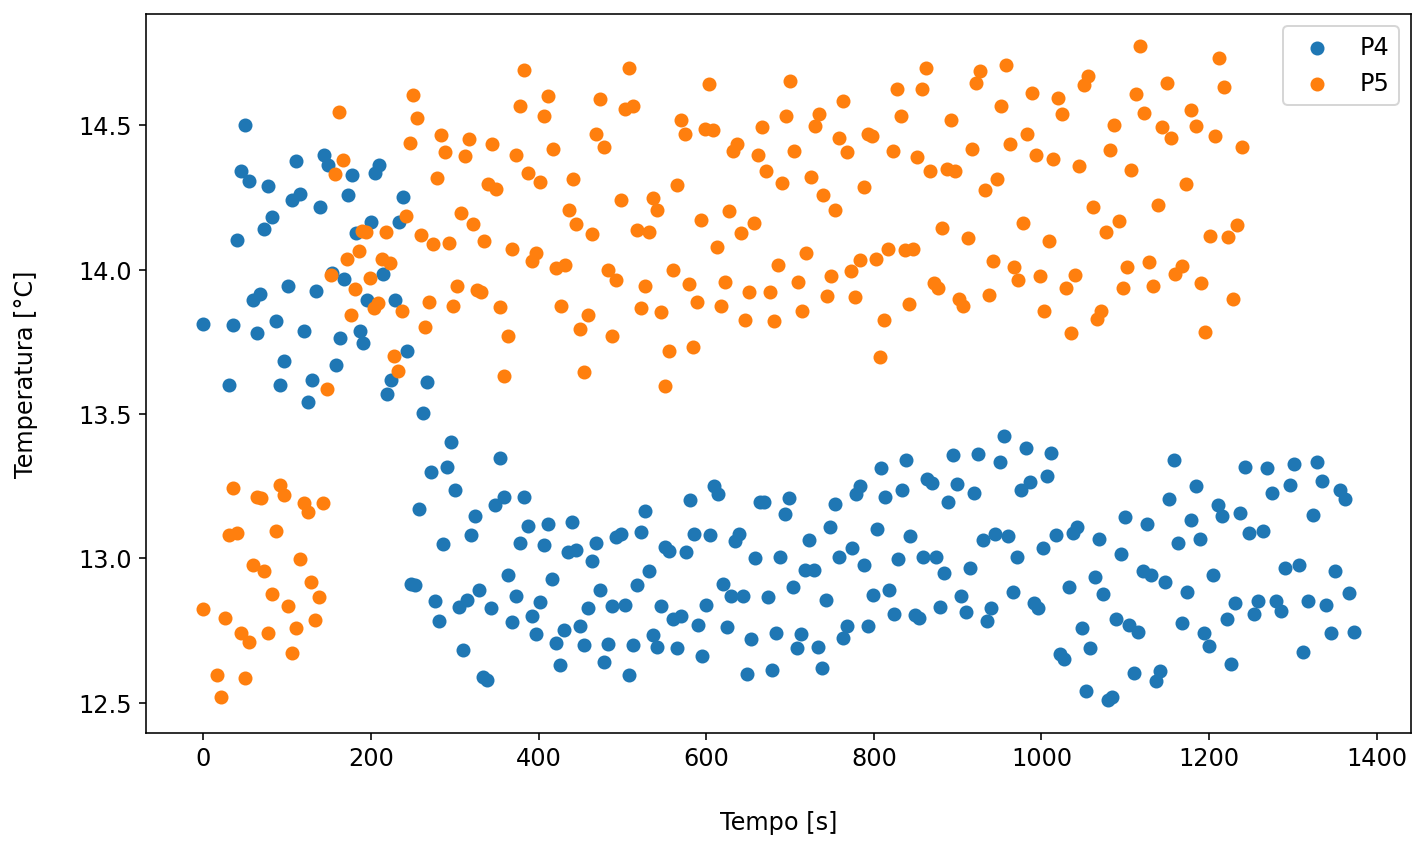
\includegraphics[width=1\linewidth]{FigurasdoTexto/Temperatura de Sucção.png}
    \caption{Temperatura de Sucção  nas Perturbações P4 e P5}
    \label{fig:TempSucçãoSubidaeDescida}
    {\footnotesize O Autor (2025)}
\end{figure}

\subsection{Análise do COP}

\subsection{Parâmetros de Controle}